\documentclass{article}
\title{Algebra II\\
\large Homework 1
}
\author{Nutan Nepal}
\usepackage{tikz, pgfplots}
\usepackage{tikz-cd}

\begin{document}
\maketitle

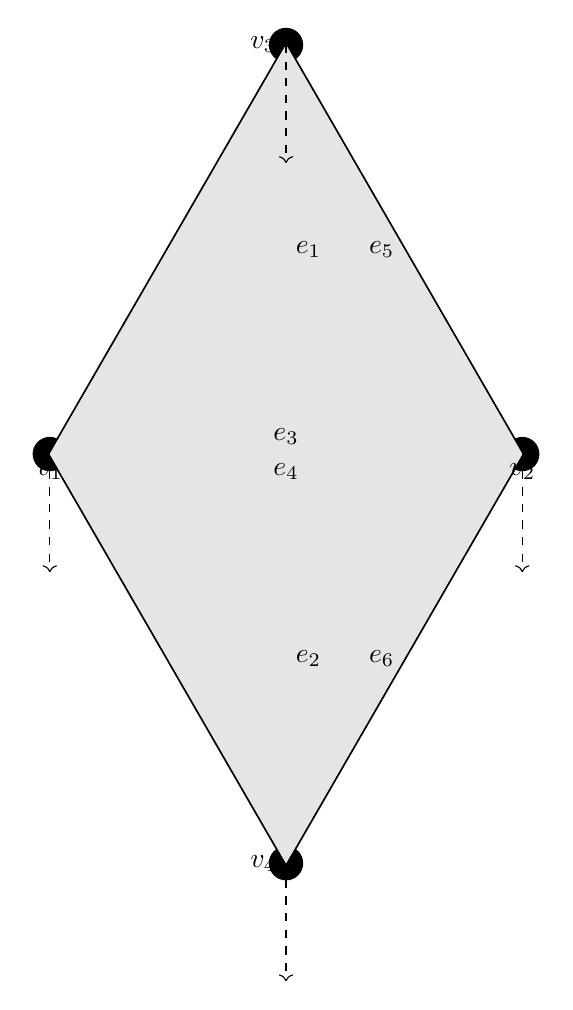
\begin{tikzpicture}[scale=3]
    % vertices
    \filldraw[black] (0,0) circle (2pt);
    \filldraw[black] (2,0) circle (2pt);
    \filldraw[black] (1,1.732) circle (2pt);
    \filldraw[black] (1,-1.732) circle (2pt);
    % edges
    \draw[black, line width=0.5mm] (0,0) -- (2,0);
    \draw[black, line width=0.5mm] (0,0) -- (1,1.732);
    \draw[black, line width=0.5mm] (0,0) -- (1,-1.732);
    \draw[black, line width=0.5mm] (2,0) -- (1,1.732);
    \draw[black, line width=0.5mm] (2,0) -- (1,-1.732);
    \draw[black, line width=0.5mm] (1,1.732) -- (1,-1.732);
    % faces
    \fill[black!10!white] (0,0) -- (2,0) -- (1,-1.732) -- cycle;
    \fill[black!10!white] (0,0) -- (2,0) -- (1,1.732) -- cycle;
    \fill[black!10!white] (0,0) -- (1,1.732) -- (1,-1.732) -- cycle;
    \fill[black!10!white] (2,0) -- (1,1.732) -- (1,-1.732) -- cycle;
    % labels
    \node[below] at (0,0) {$v_1$};
    \node[below] at (2,0) {$v_2$};
    \node[left] at (1,1.732) {$v_3$};
    \node[left] at (1,-1.732) {$v_4$};
    \node[right] at (1,0.866) {$e_1$};
    \node[right] at (1,-0.866) {$e_2$};
    \node[above] at (1,0) {$e_3$};
    \node[below] at (1,0) {$e_4$};
    \node[left] at (1.5,0.866) {$e_5$};
    \node[left] at (1.5,-0.866) {$e_6$};
    % attachments
    \draw[black, dashed, ->] (0,0) -- (0,-0.5);
    \draw[black, dashed, ->] (2,0) -- (2,-0.5);
    \draw[black, dashed, ->] (1,1.732) -- (1,1.232);
    \draw[black, dashed, ->] (1,-1.732) -- (1,-2.232);
    \end{tikzpicture}
    
\end{document}